\section{Helpfulness Prediction}
Our ambitious goal was that of building a model able to predict the helpfulness of a review, looking only at the text of the review itself.
To create such a model, we needed firstly to convert the text in a machine-readable format, performing a process called \textit{feature extraction}.
Then we tried different models, in order to find the one that best fits our needs eventually selecting the best one.

\subsection{Feature Extraction}
Seen the complexity of the problem we decided to use a \textit{Word Embedding} technique, called \textit{Word2Vec}, that is able to convert a word in a vector of real numbers
while preserving the semantic meaning of the word itself. We used the \textit{Gensim} library to perform this task using the following parameters for the model:
\begin{itemize}[noitemsep, leftmargin=*]
    \item \textbf{Size}: 30
    \item \textbf{Window}: 5
    \item \textbf{Min Count}: 2
    \item \textbf{Workers}: -1
\end{itemize}
As a consequence, each word is represented by a vector of 30 real numbers. The average of the vectors of all the words in a review is the vector representation of the review.

\subsection{Models}
We tried three different models: \textit{Random Forest}, \textit{Support Vector Regressor (RBF kernel)} and \textit{MLP}.
We used the \textit{Scikit-Learn} library to perform the training and the testing of the models. Specifically for this last step
we used the \textit{GridSearchCV} class, that performs a cross-validation on the training set, in order to find the best parameters for the model.
The results are show in Table \ref{tab:model_results} and supported by Figure \ref{fig:model_results}.

\begin{table}[H]
    \footnotesize
    \centering
    \caption{Model Results}
    \label{tab:model_results}
    \begin{tabular}{|c|c|c|c|}
        \hline
        Model & MSE & RMSE & R\textsuperscript{2} \\
        \hline
        RF & 0.0259 & 0.1609 & 0.2532 \\
        SVR & 0.0279 & 0.1670 & 0.1955 \\
        MLP & 0.0282 & 0.1680 & 0.1858 \\
        \hline
    \end{tabular}
\end{table}

\begin{figure}[H]
    \centering
    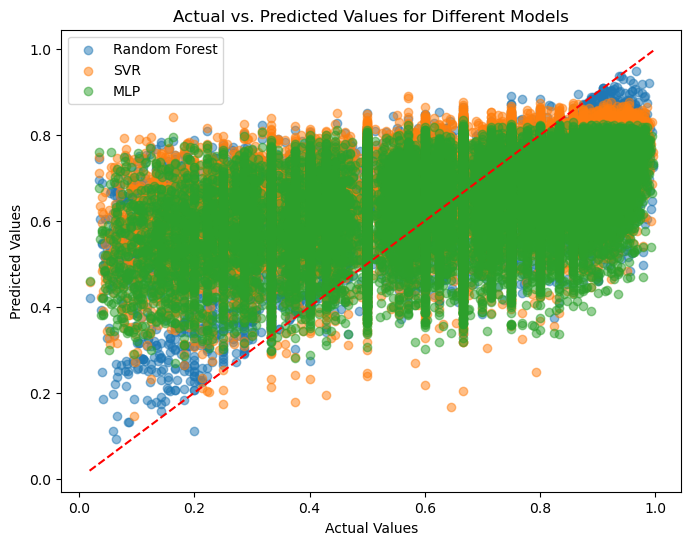
\includegraphics[width=0.48\textwidth]{./figures/model_results.png}
    \caption{Model Results}
    \label{fig:model_results}
\end{figure}

\noindent
As we can see from the graph and the metrics used, the Random Forest model outperforms the other models in terms of Mean Squared Error 
(MSE) and Root Mean Squared Error (RMSE). The Random Forest model achieved the lowest MSE of approximately 0.026 and RMSE of approximately 
0.161, indicating that its predictions are, on average, the closest to the actual values. 
This suggests that Random Forest has the best overall predictive performance among the three models.\\
To further improve the performance of the model, we tried for the best one only to increase the number of features from 30 to 150. However,
the performance improvement was not significant, thereby we decided to keep the number of features to 30 since it strikes the best balance
between performance and computational cost.

\subsection{Results Interpretation}
Figure \ref{fig:model_best_scatter} and Figure \ref{fig:model_best_lines} help us in the results Interpretation. The scatter plot
provides a visual representation of the errors distribution, showing that the model tends to overestimate the helpfulness of the reviews when 
these latter have a high helpfulness while it underestimates when the helpfulness is low. A throughout analysis of the causes of this behavior
is on top of our future work.\\

\begin{figure}[H]
    \centering
    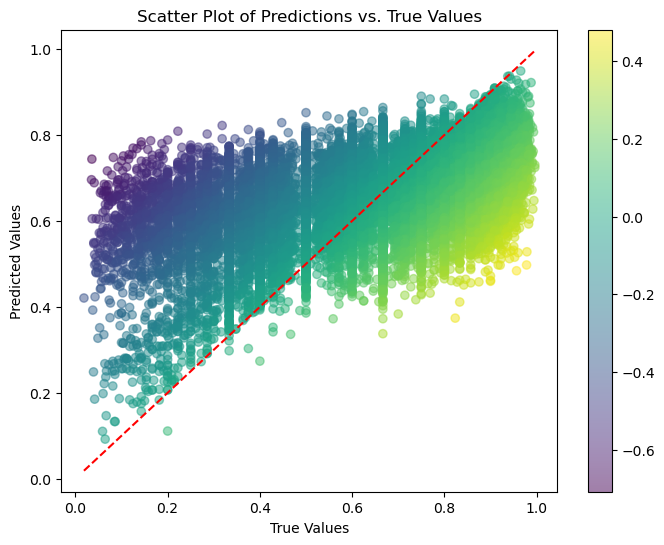
\includegraphics[width=0.48\textwidth]{./figures/model_best_scatter.png}
    \caption{Best Model Errors}
    \label{fig:model_best_scatter}
\end{figure}

\noindent
The line plot instead, helps in understanding the meaning of given helpfulness score, translating it into Total Votes and Helpfulness Votes.
The blue line represents the couple of values (Total Votes, Helpfulness Votes) leading to an helpfulness score closer to 0.8, while the red and green lines
represent the values corresponding to an helpfulness score of 0.8 plus or minus the RMSE. For example on a base of 100 Total Votes, the RMSE of 
our model corresponds to an excess or defect of roughly 13 votes.\\
\begin{figure}[H]
    \centering
    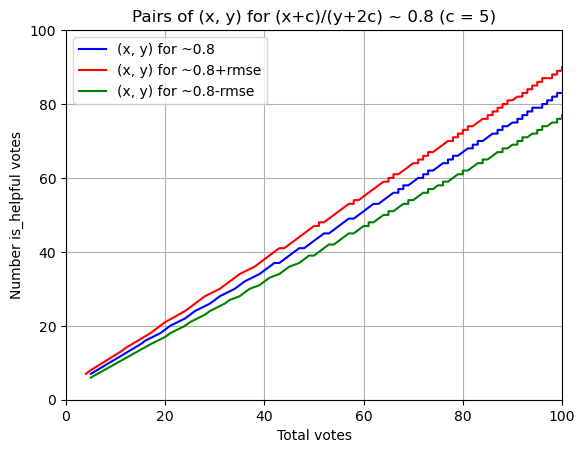
\includegraphics[width=0.48\textwidth]{./figures/model_best_lines.png}
    \caption{Best Model Errors Translation}
    \label{fig:model_best_lines}
\end{figure}




